% !TEX encoding = UTF-8 Unicode
\newpage

\chapter{Télécommande Android}
\section{Présentation Télécommande}
\lettrine[lines=1]{L}a télécommande permet par le réseau local de piloter le robot en mode semi-autonome.


La première page sur laquelle on arrive
\begin{center}
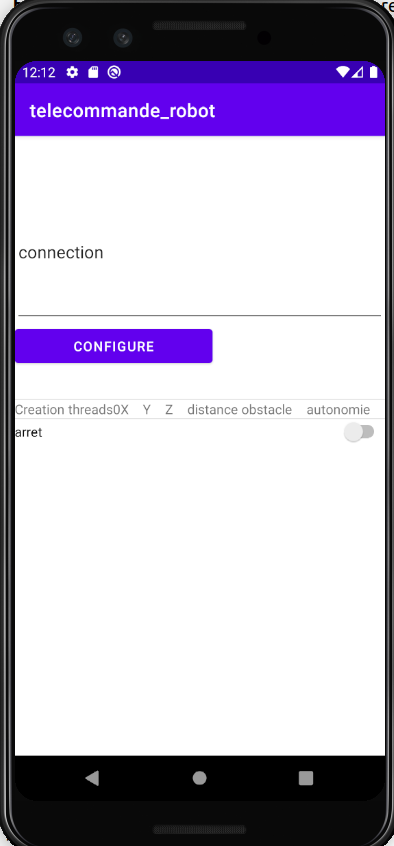
\includegraphics[width=4cm]{telecommande/page1.png} 
\end{center}

Ensuite on configure le nom d'utilisateur, le mot de passe et l'adresse du robot dans la page de configuration.

\begin{center}
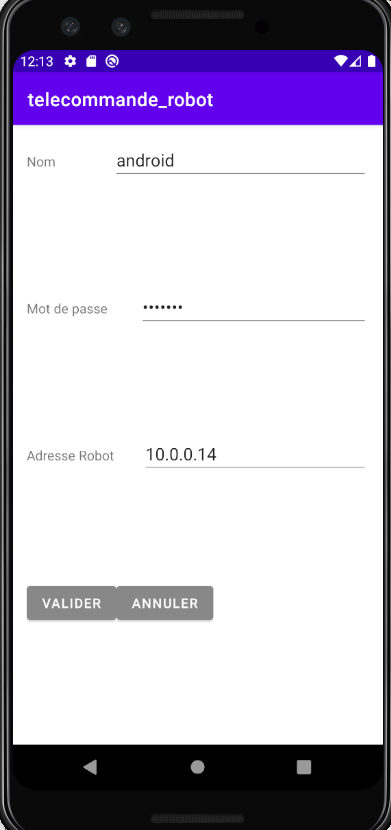
\includegraphics[width=4cm]{telecommande/configuration.png}
\end{center}

Une fois les paramètres de configuration validés, on revient sur la page de commande du robot. On appuie sur connecte, et si la connection avec le robt est établie, les boutons de pilotages apparaissent.

\begin{center}
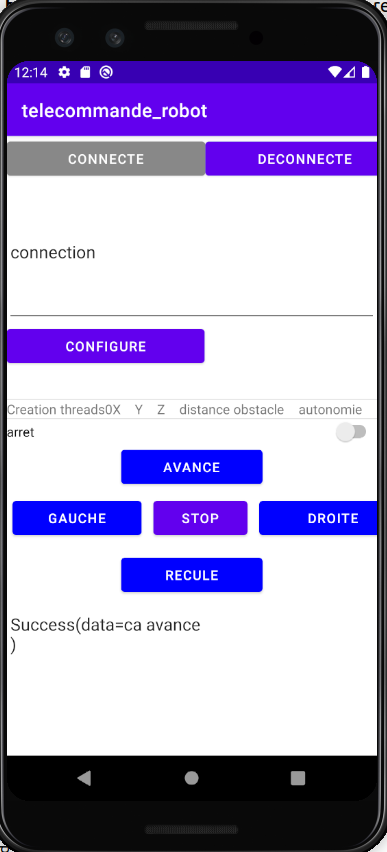
\includegraphics[width=4cm]{telecommande/telecommande.png} 
\end{center} 	
	
 \end{figure}
 